\section{Method}
\label{sec:method}

\subsection{Background: ColBERT and MaxSim Retrieval}
\label{sec:method-background}

Late-interaction retrieval, introduced by ColBERT \citep{khattab2020colbert}, scores query-document pairs at the level of individual token vectors. Given a query $Q$ and document $D$, an encoder $E_\theta$ produces sequences of token vectors $\{q_i\}_{i=1}^{|Q|}$ and $\{d_j\}_{j=1}^{|D|}$, each projected to dimension $k$ and $L_2$-normalized. The relevance score is the sum over query tokens of the best matching cosine similarity in the document:
\begin{equation}
\label{eq:maxsim}
\mathrm{score}(Q, D) = \sum_{i=1}^{|Q|} \max_{1 \le j \le |D|} \langle q_i, d_j \rangle.
\end{equation}
We follow the standard cross-lingual ColBERT setup: an XLM-RoBERTa encoder with a 128-dimensional linear projection \citep{conneau2020xlmr}. The model is trained with symmetric in-batch InfoNCE \citep{gao2021simcse,wang2020understanding} over aligned source-target pairs:
\begin{equation}
\label{eq:infonce}
\mathcal{L}_{\mathrm{InfoNCE}} = \tfrac{1}{2}\bigl[ \ell(S, T) + \ell(T, S) \bigr],
\end{equation}
where $\ell(S, T)$ is the cross-entropy of the temperature-scaled scores from \eqref{eq:maxsim} against the diagonal positive assignment. Concretely, we compute a single $B \times B$ MaxSim score matrix with source tokens as queries and target tokens as documents, and apply symmetric cross-entropy along both axes by transposing this matrix; because \eqref{eq:maxsim} is asymmetric in its query and document arguments, this is not identical to recomputing MaxSim with target tokens as queries. We use the transposed form throughout — the same symmetric-cross-entropy pattern standard in CLIP-style contrastive pretraining.

\subsection{Token-Level Anisotropy}
\label{sec:method-anisotropy}

Anisotropy in single-vector encoders refers to the empirical observation that contextual embeddings concentrate in a narrow cone of the hypersphere, with mean cosine similarity between random vectors well above zero \citep{ethayarajh2019contextual,gao2019representation,mu2018allbutthetop}. For sentence-pooled representations, the consequences are partially masked: pooling averages over tokens and downstream similarity is computed once per pair. Late-interaction scoring is qualitatively different. Every query token participates in \eqref{eq:maxsim} through a hard argmax, so the score depends on the angular separation between many candidate token directions.

We quantify token-level anisotropy with two metrics computed on a fixed pool of valid (non-pad) token vectors $X \in \mathbb{R}^{N \times k}$:

\paragraph{Intra-cosine similarity.} The mean off-diagonal cosine similarity,
\begin{equation}
\label{eq:intracos}
\mathrm{IC}(X) = \frac{1}{N(N-1)} \sum_{i \ne j} \langle x_i, x_j \rangle.
\end{equation}
A value near zero indicates an isotropic spread; values close to one indicate collapse.

\paragraph{Effective rank.} The exponential entropy of the normalized singular value distribution \citep{wang2020understanding}: given singular values $\sigma_1, \ldots, \sigma_k$ of $X$ and probabilities $p_i = \sigma_i / \sum_j \sigma_j$,
\begin{equation}
\label{eq:erank}
\mathrm{eRank}(X) = \exp\!\Bigl( - \sum_{i=1}^{k} p_i \log p_i \Bigr).
\end{equation}
Effective rank counts the number of dimensions that the embedding space actively uses; collapse pulls it toward 1.

We will show in Section~\ref{sec:results} that token vectors of multilingual ColBERT trained with vanilla InfoNCE exhibit intra-cosine of $0.20$ on English tokens and $0.29$ on Spanish tokens, with effective rank below $106$ out of a possible $128$. The asymmetry is consistent with the geometry of bitext contrastive training: in an English-Spanish pair, the Spanish side carries most of the contrastive gradient pressure and so collapses harder.

\begin{figure}[t]
\centering
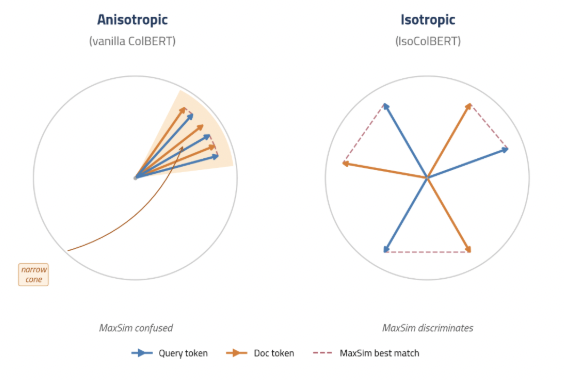
\includegraphics[width=0.95\columnwidth]{figs/fig_idea.png}
\caption{Effect of token-level anisotropy on MaxSim retrieval. Left: under vanilla training, token vectors concentrate in a narrow cone, so query tokens and document tokens have similar cosine similarity to many candidates and MaxSim cannot cleanly discriminate the true match. Right: under IsoColBERT, tokens spread across the hypersphere, giving MaxSim a larger margin between the true match and confusers.}
\label{fig:idea}
\end{figure}

\subsection{The IsoColBERT Objective}
\label{sec:method-iso}

If token-level anisotropy degrades MaxSim, the natural remedy is to add a training-time penalty that pushes token vectors apart. We define a per-batch isotropy regularizer that penalizes the squared off-diagonal cosine similarities of the valid token vectors in the batch:
\begin{equation}
\label{eq:reg}
R(X) = \frac{1}{N(N-1)} \sum_{i \ne j} \langle x_i, x_j \rangle^2.
\end{equation}
The squared form has two properties we want. It is non-negative, with its minimum attained when all pairs are orthogonal. We do not reach this minimum in practice: with $N \le 256$ token vectors subsampled into $k=128$ dimensions, at most $k$ pooled vectors can be mutually orthogonal, so the exact zero is unattainable in our setting. The loss nonetheless continues to drive pairwise cosine similarities toward zero, spreading the pooled vectors as far apart as the embedding dimension permits. The squared form also penalizes negative correlations as well as positive ones, which is appropriate on the hypersphere where $\langle x_i, x_j \rangle$ already takes values in $[-1, 1]$.

The full IsoColBERT objective adds \eqref{eq:reg} to the InfoNCE loss with weight $\lambda$, applied symmetrically to the query and document token banks:
\begin{equation}
\label{eq:loss}
\mathcal{L} = \mathcal{L}_{\mathrm{InfoNCE}} + \lambda \cdot \tfrac{1}{2}\bigl( R(X_Q) + R(X_D) \bigr).
\end{equation}
$X_Q$ and $X_D$ are the pooled valid token matrices for queries and documents in the current mini-batch. The regularizer has a single hyperparameter and no architectural change, so it adds zero cost at inference time.

\subsection{Connection to Uniformity}
\label{sec:method-uniformity}

\citet{wang2020understanding} decompose the asymptotic InfoNCE loss into an alignment term (positives close) and a uniformity term (features spread on the hypersphere). Their uniformity term penalizes pairwise Gaussian potentials $\exp(-t\,\|x_i - x_j\|^2)$, which for $L_2$-normalized vectors is monotonic in $\langle x_i, x_j \rangle$. Our regularizer \eqref{eq:reg} is a token-level analog of this uniformity penalty, applied inside sequence models where the contrastive objective operates over sentence-pooled vectors rather than individual tokens. \citet{xiao2023isotropy} observe that InfoNCE alone already partially induces isotropy in sentence encoders; our results in Section~\ref{sec:results} show that for multilingual late-interaction retrieval, the implicit pressure from InfoNCE is insufficient and explicit token-level regularization adds substantial value.

We frame the role of regularization for MaxSim as follows. The hard argmax in \eqref{eq:maxsim} routes the score gradient through a single best-matching document token per query token. When the embedding space is anisotropic, many candidate document tokens have similar cosine similarity to the query token, so the argmax is unstable and the score depends weakly on the identity of the true match. Spreading token vectors across more of the hypersphere increases the cosine margin between the true match and confusers, which may increase the margin available to MaxSim.

\subsection{Implementation}
\label{sec:method-impl}

On each training step, we pool the valid (non-pad) token vectors of all queries in the batch into $X_Q \in \mathbb{R}^{N_Q \times k}$, and similarly $X_D \in \mathbb{R}^{N_D \times k}$. For efficiency at large batch sizes we subsample up to $256$ tokens per side. We compute the Gram matrix $G = X X^\top \in \mathbb{R}^{N \times N}$ (whose off-diagonal entries are the pairwise cosine similarities, since $X$ is row-normalized) and evaluate the regularizer as the mean of the squared off-diagonal entries: $R(X) = \bigl(\|G\|_F^2 - \sum_i G_{ii}^2\bigr) \big/ \bigl(N(N-1)\bigr)$. With $L_2$-normalized rows $G_{ii}=1$, so this reduces to $\bigl(\|G\|_F^2 - N\bigr) \big/ \bigl(N(N-1)\bigr)$, computed via a single matmul plus a trace subtraction. The regularizer adds one additional matmul per step at training time and is removed entirely at inference: the inference graph is identical to a vanilla ColBERT encoder. Algorithm~\ref{alg:training} summarizes the procedure. We compare this uniform placement against two alternative placements in Section~\ref{sec:ablations} to isolate which part of the token manifold matters.

\begin{algorithm}[t]
\caption{IsoColBERT training step}
\label{alg:training}
\begin{algorithmic}[1]
\REQUIRE Batch of paired sentences $\{(s_i, t_i)\}_{i=1}^B$; encoder $E_\theta$; temperature $\tau$; regularizer weight $\lambda$.
\STATE $(\{q_i\}, M_Q) \leftarrow E_\theta(\{s_i\})$ \COMMENT{query token vectors and validity masks}
\STATE $(\{d_i\}, M_D) \leftarrow E_\theta(\{t_i\})$
\STATE $S_{ij} \leftarrow \tau^{-1} \sum_t M_Q^{(t)} \max_{u: M_D^{(u)} = 1} \langle q_i^{(t)}, d_j^{(u)} \rangle$ for all $(i, j)$ \COMMENT{MaxSim, with padding tokens excluded on both sides}
\STATE $\mathcal{L}_{\mathrm{InfoNCE}} \leftarrow \tfrac{1}{2}\bigl(\mathrm{CE}(S, \mathbf{I}) + \mathrm{CE}(S^\top, \mathbf{I})\bigr)$
\IF{$\lambda > 0$}
  \STATE $X_Q \leftarrow$ pooled valid query tokens (up to 256)
  \STATE $X_D \leftarrow$ pooled valid document tokens (up to 256)
  \STATE $\mathcal{L}_{\mathrm{iso}} \leftarrow \tfrac{1}{2}\bigl(R(X_Q) + R(X_D)\bigr)$ via Eq.~\eqref{eq:reg}
\ELSE
  \STATE $\mathcal{L}_{\mathrm{iso}} \leftarrow 0$
\ENDIF
\STATE Backpropagate $\mathcal{L}_{\mathrm{InfoNCE}} + \lambda \cdot \mathcal{L}_{\mathrm{iso}}$ through $\theta$.
\end{algorithmic}
\end{algorithm}

\paragraph{Computational overhead.} The regularizer adds one additional matrix multiplication per training step on each of the query and document sides: forming the Gram matrix $G = XX^\top$ for the pooled token bank of size $N \le 256$ at projection dimension $k=128$ costs $\Theta(N^2 k)$ floating-point operations, at most $\approx 17$M per side. The Frobenius and trace terms that derive $R(X)$ from $G$ are $\Theta(N^2)$ and $\Theta(N)$ respectively and contribute negligibly. By contrast, a single XLM-RoBERTa-base forward pass at sequence length $L=64$, hidden dimension $d_{\text{model}}=768$, and feed-forward dimension $d_{\text{ff}}=3072$ costs $\Theta(L \cdot d_{\text{model}}^2 + L^2 \cdot d_{\text{model}} + L \cdot d_{\text{model}} \cdot d_{\text{ff}})$ per layer over $12$ layers \citep{conneau2020xlmr}. At the effective batch size of $32$ used in our experiments, the encoder forward pass on the joint query and document sides exceeds the regularizer's cost by more than three orders of magnitude, so the regularizer is well within the noise of a typical training step. At inference the regularizer is removed entirely: there are no extra parameters, no extra FLOPs, and the deployment graph is identical to a vanilla ColBERT encoder.

\paragraph{Alternative placements.} Two natural variants restrict where the regularizer applies. The \emph{active-token} variant regularizes only the tokens that win MaxSim (each query token and its argmax document token). The \emph{cross-attention} variant penalizes redundancy in the $L_q \times L_d$ MaxSim score matrix itself rather than the underlying token vectors. We define these formally and report their performance in Section~\ref{sec:ablations}.
